\begin{song}{Čarodějnice z Amesbury}{F}{Asonance}
  \begin{SBVerse}
    Zuzana \Ch{dmi}{byla} dívka, \Ch{C}{která} žila v \Ch{dmi}{Ame}sbury,

s jasnýma \Ch{F}{očima} a \Ch{C}{řečmi} pánům \Ch{dmi}{navzdo}ry,

souse\Ch{F}{dé} o ní \Ch{C}{říka}li, že \Ch{dmi}{temná} kouzla \Ch{ami}{zná}

a \Ch{Bb}{že} se lidem \Ch{ami}{vyhýbá} a s \Ch{Bb}{ďáblem} \Ch{C}{pletky} \Ch{dmi(G)}{má.}

  \end{SBVerse}

  \begin{SBVerse}
Onoho léta náhle mor dobytek zachvátil

a pověrčivý lid se na pastora obrátil,

že znají tu moc nečistou, jež krávy zabíjí,

a odkud ta moc vychází, to každý dobře ví.

  \end{SBVerse}

  \begin{SBVerse}
Tak Zuzanu hned před tribunál předvést nechali,

a když ji vedli městem, všichni kolem volali:

"Už konec je s tvým řáděním, už nám neuškodíš,

teď na své cestě poslední do pekla poletíš!"

  \end{SBVerse}

  \begin{SBVerse}
Dosvědčil jeden sedlák, že zná její umění,

ďábelským kouzlem prý se v netopýra promění

a v noci nad krajinou létává pod černou oblohou,

sedlákům krávy zabíjí tou mocí čarovnou.

  \end{SBVerse}

  \begin{SBVerse}
Jiný zas na kříž přísahal, že její kouzla zná,

v noci se v černou kočku mění dívka líbezná,

je třeba jednou provždy ukončit ďábelské řádění,

a všichni křičeli jako posedlí:"Na šibenici s ní!"

  \end{SBVerse}

  \begin{SBVerse}
Spektrální důkazy pečlivě byly zváženy,

pak z tribunálu povstal starý soudce vážený:

"Je přece v knize psáno: nenecháš čarodějnici žít

a před ďáblovým učením budeš se na pozoru mít!"

  \end{SBVerse}

  \begin{SBVerse}
Zuzana stála krásná s hlavou hrdě vztyčenou

a její slova zněla klenbou s tichou ozvěnou:

"Pohrdám vámi, neznáte nic nežli samou lež a klam,

pro tvrdost vašich srdcí jen, jen pro ni umírám!"

  \end{SBVerse}

  \begin{SBVerse}
Tak vzali Zuzanu na kopec pod šibenici

a všude kolem ní se sběhly davy běsnící,

a ona stála bezbranná, však s hlavou vztyčenou,

zemřela tiše samotná pod letní oblohou ...


  \end{SBVerse}
  \begin{center}
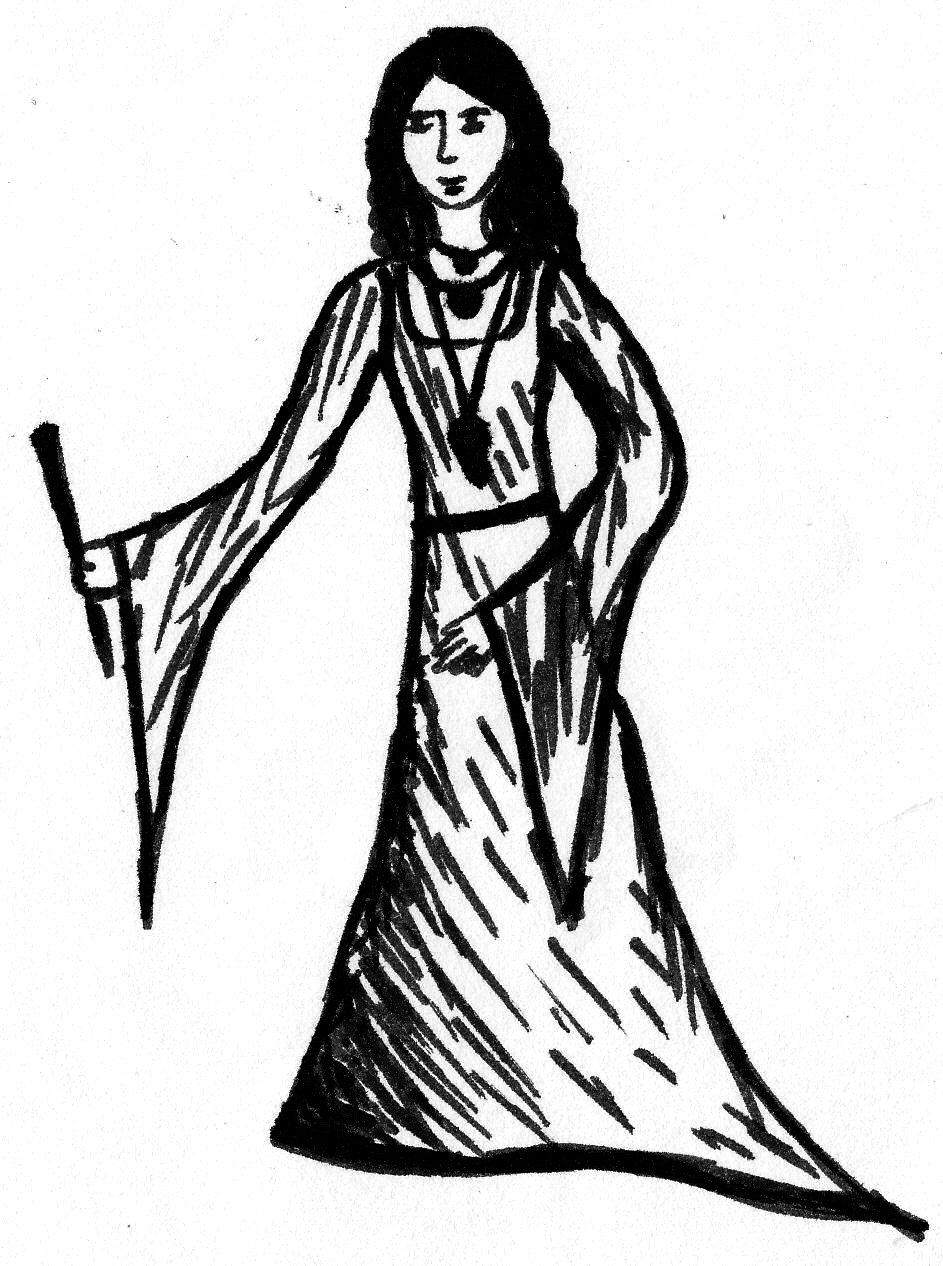
\includegraphics[width=5cm]{pict/carodejnice_z_amesbury}
\end{center}
\end{song}
\pagebreak
